Consider the $m$-degree polynomial $P(m, X, N)$ having fixed non-negative integers $m$ and $N$
\begin{align*}
    P(m,X,N) = \sum_{r=0}^{m} \sum_{k=1}^{N} \coeffA{m}{r} k^r (X-k)^r
\end{align*}
For example
\begin{align*}
    P(2,X,0) &= 0 \\
    P(2,X,1) &= 30X^2 - 60X + 31 \\
    P(2,X,2) &= 150X^2 - 540X + 512 \\
    P(2,X,3) &= 420X^2 - 2160X + 2943 \\
    P(2,X,4) &= 900X^2 - 6000X + 10624
\end{align*}
where $\coeffA{m}{r}$ is a real coefficient defined recursively, see~\cite{alekseyev2018mathoverflow,
    on_the_link_between_binomial_theorem_and_discrete_convolution, unusual_identity_for_odd_powers,
    history_and_overview_of_polynomial_p}.
For example,
\begin{table}[H]
    \begin{center}
        \setlength\extrarowheight{-6pt}
        \begin{tabular}{c|cccccccc}
            $m/r$ & 0 & 1       & 2      & 3      & 4   & 5    & 6     & 7 \\ [3px]
            \hline
            0     & 1 &         &        &        &     &      &       &       \\
            1     & 1 & 6       &        &        &     &      &       &       \\
            2     & 1 & 0       & 30     &        &     &      &       &       \\
            3     & 1 & -14     & 0      & 140    &     &      &       &       \\
            4     & 1 & -120    & 0      & 0      & 630 &      &       &       \\
            5     & 1 & -1386   & 660    & 0      & 0   & 2772 &       &       \\
            6     & 1 & -21840  & 18018  & 0      & 0   & 0    & 12012 &       \\
            7     & 1 & -450054 & 491400 & -60060 & 0   & 0    & 0     & 51480
        \end{tabular}
    \end{center}
    \caption{Coefficients $\coeffA{m}{r}$. See OEIS sequences
    ~\cite{oeis_numerators_of_the_coefficient_a_m_r,oeis_denominators_of_the_coefficient_a_m_r}.}
    \label{tab:table_of_coefficients_a}
\end{table}


In this manuscript we discuss approximation properties of polynomial $P(m,X,N)$.
I use a few well-known criteria to measure and estimate error of approximation: Absolute error, Relative error and
Percentage error.
Assume that function $f_2(x)$ approximates the function $f_1 (x)$ then the errors are

\begin{align*}
    \mathrm{Absolute \; Error}   &= \frac{\lvert f_1(x) - f_2(x) \rvert}{\lvert f_1(x) \rvert} \\
    \mathrm{Relative \; Error}   &= \frac{\lvert f_1(x) - f_2(x) \rvert}{\lvert f_1(x) \rvert} \\
    \mathrm{Percentage \; Error} &= \frac{\lvert f_1(x) - f_2(x) \rvert}{\lvert f_1(x) \rvert} \times 100\%
\end{align*}

Diving straight to the point, we switch our focus to already mentioned polynomial $P(2,X,4) = 900X^2 - 6000X + 10624$
to show the first example of how it approximates the odd power function $X^5$.
In fact, we approximate the polynomial $X^{2m+1}$ by lower degree polynomial $X^m$ as the following image presents
\begin{figure}[H]
    \centering
    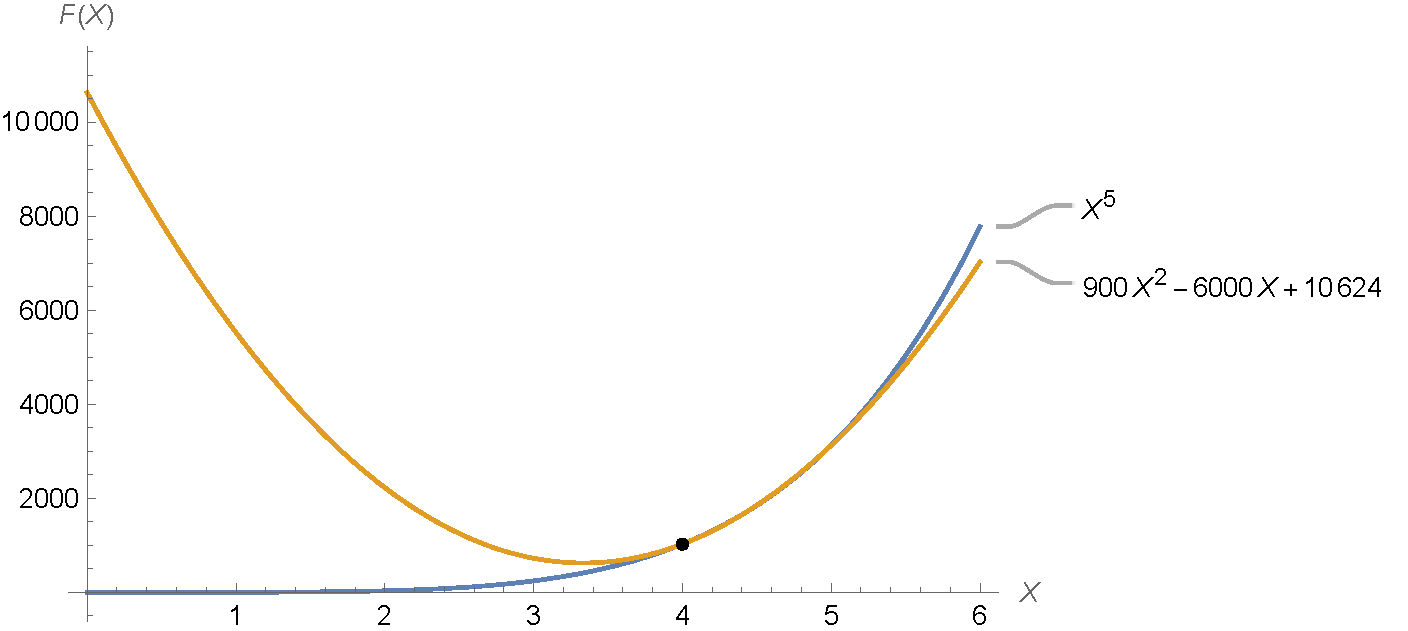
\includegraphics[width=1\textwidth]{sections/images/03_plots_polynomial_p2_n4_with_fifth}
    ~\caption{Polynomial plot $P(2, X, 4)$ with fifth power $X^5$.
    Points of intersection $X=4$, $X=4.42472$, $X=4.99181$.
    Interval of convergence: $3.9 \leq X \leq 5.3$ with $E < 2\%$.
    }\label{fig:03_plots_polynomial_p2_n4_with_fifth}
\end{figure}
As we see, the interval $3.9 \leq X \leq 5.3$ has the percentage error lesser than $2\%$ which is quite impressive.
So that having fixed $N=4$ the polynomial $P(2, X, 4)$ approximates odd power in neighborhood of $N=4$
which is $3.9 \leq X \leq 5.3$.
To showcase the concrete values of absolute, relative and percentage errors of approximation above, I attach a separate
table in addenda.

One more interesting observation can be done by increasing the value of $N$ in $P(m, X, N)$ having fixed $m$, it
follows that by increasing $N$ the interval of convergence with odd-power $X^{2m+1}$ increasing as well.
For instance,
\begin{itemize}
    \item Having $P(2, X, 4)$ the interval of convergence with percentage error lesser than $1\%$ is $4.0 \leq X \leq 5.1$
    \item Having $P(2, X, 20)$ the interval of convergence with percentage error lesser than $1\%$ is $18.7 \leq X \leq 22.9$
    \item Having $P(2, X, 120)$ the interval of convergence with percentage error lesser than $1\%$ is $110.0 \leq X \leq 134.7$
\end{itemize}
